\chapter{Tables and figures}
\label{ch:tables-figures}

\section{Tables}\label{tables}

A \texttt{tabular} builds the grid, and a \texttt{table} around it adds a caption and lets it float to a good position. The \texttt{booktabs} package gives clean horizontal rules, and it\textquotesingle s best to avoid vertical lines altogether.

\begin{lstlisting}[language=latex]
\begin{table}[ht]
  \centering
  \caption{Heat loss through a wall.}
  \label{tab:walls}
  \begin{tabular}{lrr}      % left, right, right
    \toprule
    Wall & $U$ & $Q$ \\
    \midrule
    Solid brick & 2.10 & 315 \\
    Insulated   & 0.45 & 68 \\
    \bottomrule
  \end{tabular}
\end{table}
\end{lstlisting}

\begin{figure}
\centering
\includegraphics[width=\linewidth]{img/table.png}
\caption{The table in the \href{../references/}{complete report}, with three walls. Note the horizontal rules, and no vertical ones.}
\end{figure}

\section{Figures}\label{figures}

\begin{lstlisting}[language=latex]
\usepackage{graphicx}

\begin{figure}[ht]
  \centering
  \includegraphics[width=0.8\linewidth]{figures/map.pdf}
  \caption{Heat loss across the study area.}
  \label{fig:map}
\end{figure}
\end{lstlisting}

Use PDF or SVG-derived vector files for plots, as they stay sharp at any size. Use PNG for images at 300 dpi or more for print.

\section{Plots drawn from data}\label{plots-drawn-from-data}

\texttt{pgfplots} draws a chart directly in LaTeX, so its fonts match the document.

\begin{lstlisting}[language=latex]
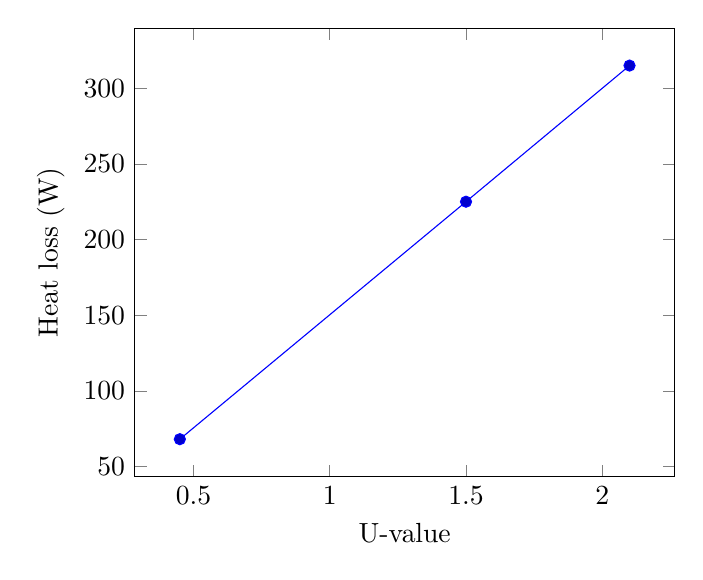
\begin{tikzpicture}
  \begin{axis}[xlabel={U-value}, ylabel={Heat loss (W)}]
    \addplot coordinates {(0.45,68) (1.5,225) (2.1,315)};
  \end{axis}
\end{tikzpicture}
\end{lstlisting}

\begin{figure}
\centering
\includegraphics[width=\linewidth]{img/figure.png}
\caption{The same plot compiled in the complete report. Its labels use the same font as the text.}
\end{figure}

For anything complex, generate the figure with a script, such as Python with Matplotlib, and include the file. Then the figure can be rebuilt from its data.

\section{Introducing them properly}\label{introducing-them-properly}

Every table and figure should be mentioned in the text before it appears, and each needs a caption that says what it shows. Put the \texttt{\textbackslash{}label} after the \texttt{\textbackslash{}caption}, or the reference will point to the section number instead. Floats move: \texttt{{[}ht{]}} asks for here or the top of a page, which is why you should refer to "Table 1" and not "the table below".

